\section{Dexterity Network}
\seclabel{dexnet}
\TODO{Due to space, it might make sense to discuss in experiments as appears to be common practice when the dataset is not going to be released to the public}
It remains to describe the details of creating the Dexterity Network (Dex-Net), our prior dataset of objects and grasps with similarity, for use in the Multi-Armed Bandit models of Algorithm~\ref{alg:full}.
Dex-Net 1.0 consists of approximately 20,162 3D mesh models \TODO{Update with correct count} collected from the datasets described in \figref{datasets}.
Laser-scanned models from the KIT object database~\cite{kasper2012kit}, the Amazon Picking Challenge objects, BigBIRD~\cite{singh2014bigbird}, and YCB ~\cite{calli2015benchmarking} constitute 355 of the total models.
These models were chosen to reflect physical objects commonly used for benchmarking in grasping research for potential future physical experiments using Dex-Net.
The majority of Dex-Net is synthetic 3D mesh models from 3DNet\cite{wohlkinger20123dnet}, a benchmark for object detection in robotics research,  ModelNet~\cite{wu20143d}, a relatively new benchmark for 3D model classification, and the SHREC 2014 large scale object retrieval challenge~\cite{li2015comparison}, a competition benchmark with many categories to test the state-of-the-art in shape retrieval annually.
While the geometry of synthetic models does not necessarily reflect a physical object, using these models allows us to examine the effects of scale at tens of thousands of 3D models, which has not been previously attempted in grasp synthesis research.

In order to use the models for grasp selection, we first preprocess each model.
Each object in Dex-Net is originally specified as a 3D mesh $\mS = \{\mV, \mT\}$ where $\mV = \{\bv_1, ..., \bv_V\}$ is a set of $V$ vertices such that $\bv_i \in \bR^3$ for $i = 1, ..., V$ and $\mT = \{t_1, ..., t_F\}$  is a set of $F$ triangles such that $t_j \in \mathbb{Z}_{+}^3$ for $j = 1, ..., F$.
First, we remove unreferenced vertices and illegal triangles (e.g. same vertex is referenced twice in one triangle).
Next, we normalize the orientation of the model by performing Principal Component Analysis (PCA) on the raw vertices of the mesh and then rotating the object such that its first principal component aligns with the $z$-axis and its second aligns with the $y$-axis.
We then set the object center of mass $\bz$ to be the center of the bounding box for the reoriented mesh.
Since synthetic models may not be specified in meters, we also rescale each mesh such that the smallest dimension of the bounding box lies withing the maximum opening of the gripper.
Finally, we convert each mesh to a signed distance field $f$ using SDFGen~\cite{}, an open-source C++ tool.

Once each 3D model is preprocessed, we compute the shape feature vector described in \secref{cnn} for each object.
Each feature vector is then put into a KD-Tree nearest neighbor query structure for accelerated lookups of shape nearest neighbors.
This structure consistutes our shape similiarity network, in which each object $\mO$  is connected to its $n$ nearest neighbors $\mO_1, ..., \mO_n$ by an edge of weight $\| \psi(\mO) - \psi(\mO_i) \|_2^2$.
We generate a set of grasps for each object in the network using the method of \secref{candidates} and evaluate the probability of force closure for each grasp using brute-force Monte Carlo integration as a benchmark~\cite{kehoe2012toward}.
As the number of models is quite large, we distribute the grasp labelling for each object across virtual machines in Google Compute Engine and aggregate the results at the end.


\begin{figure}[t!]
\centering
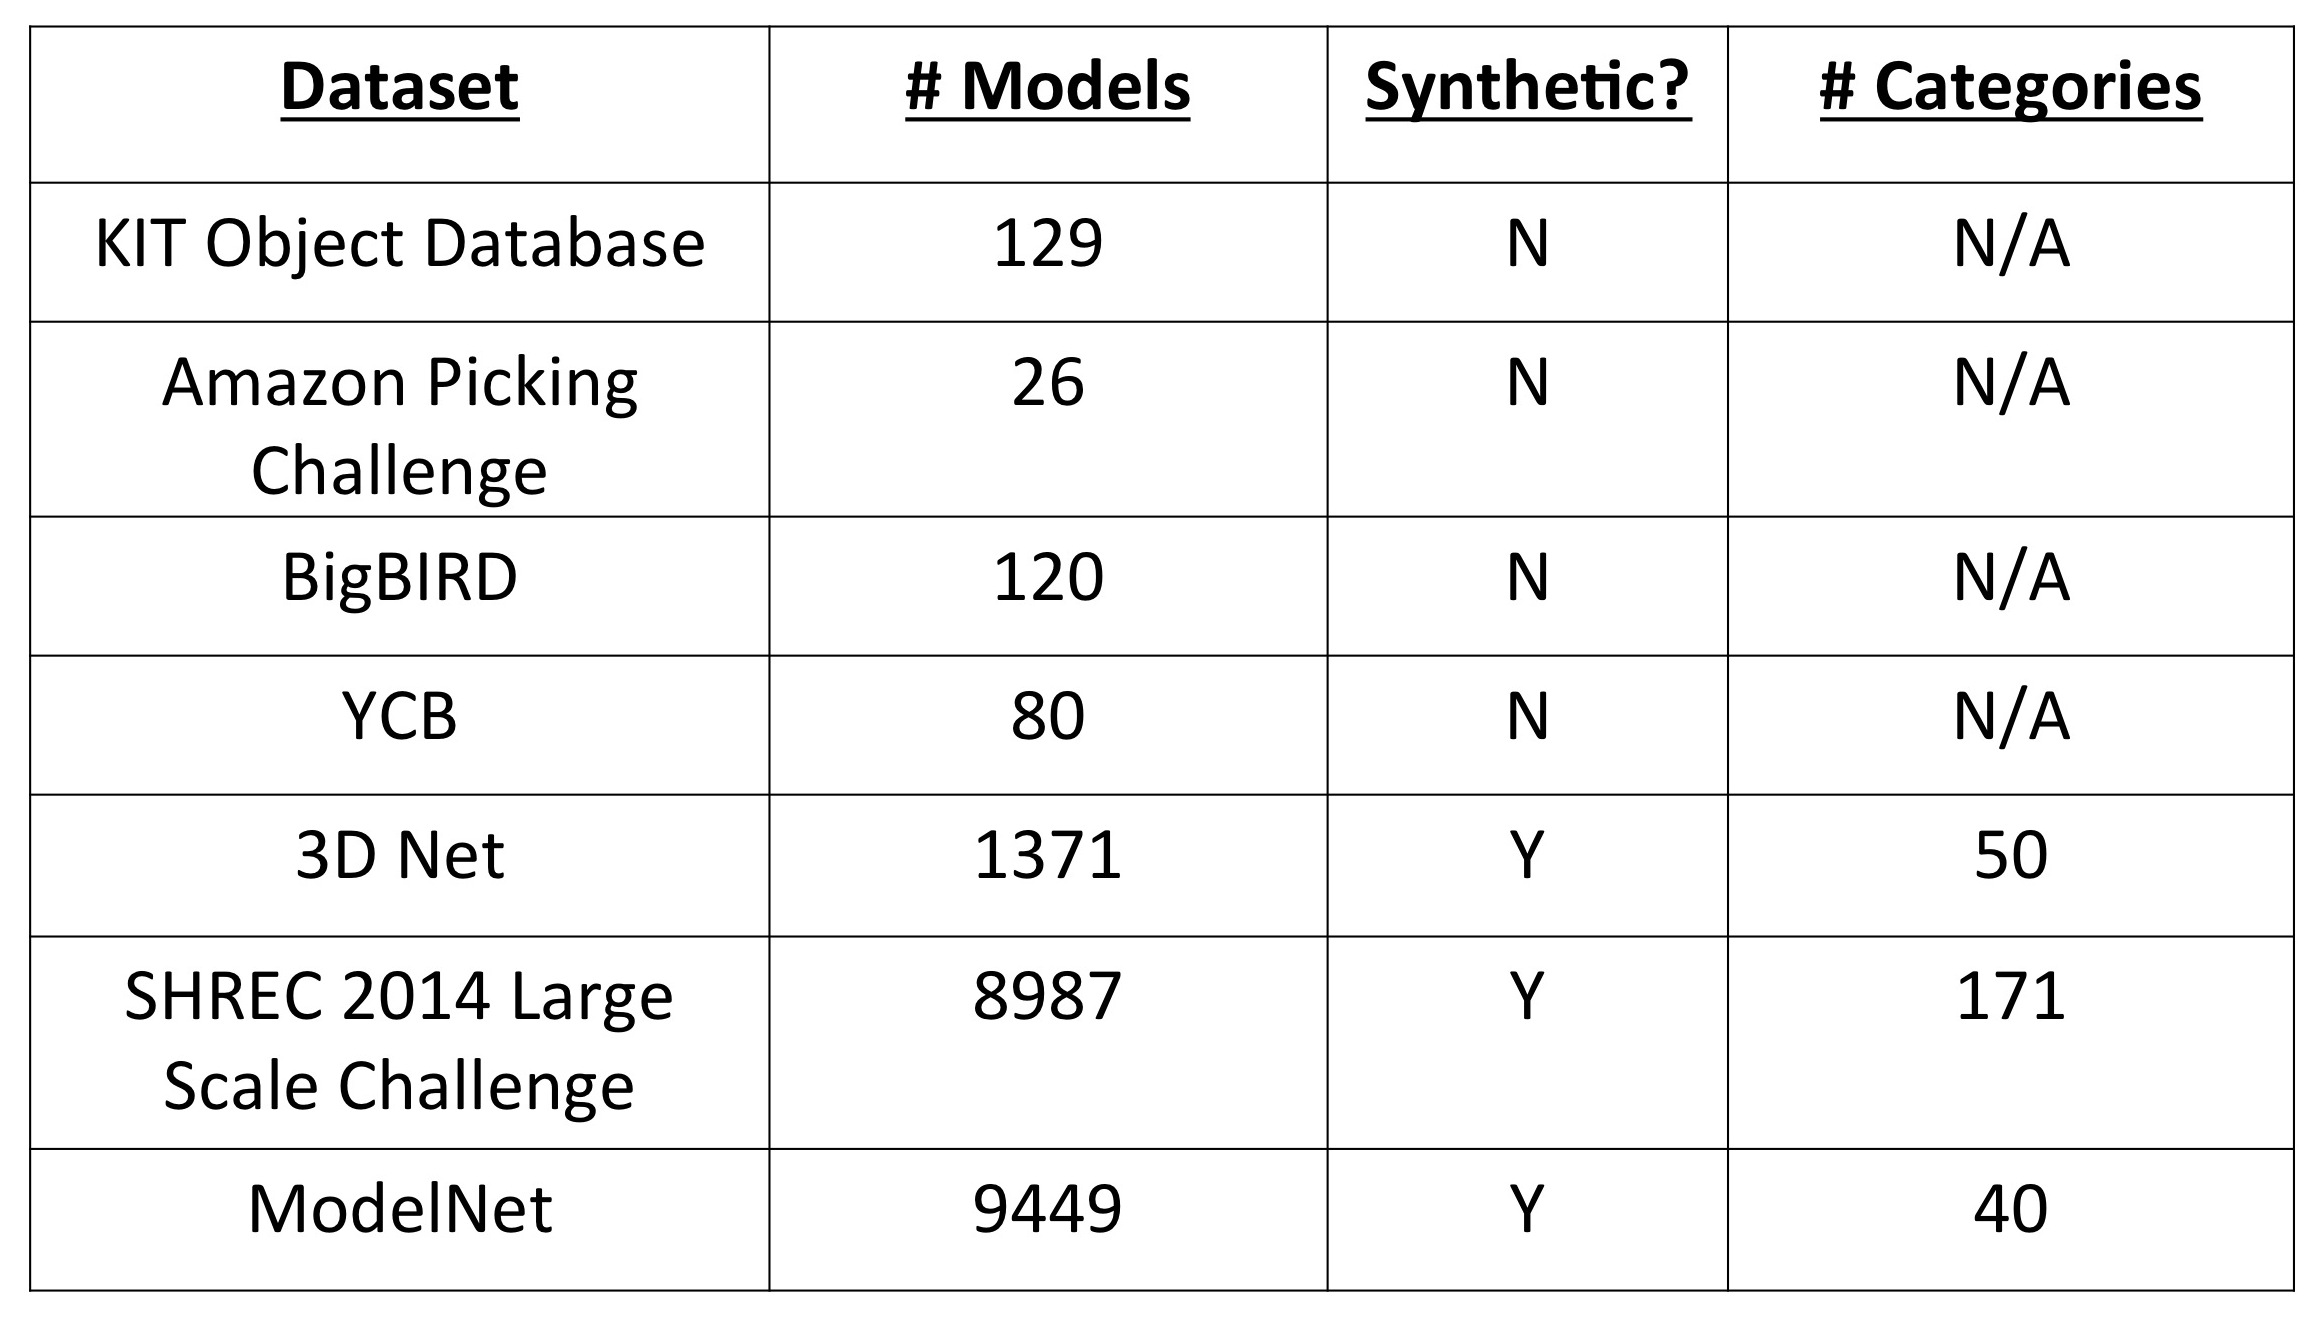
\includegraphics[scale=0.1]{figures/dataset_table.jpg}
\caption{The seven datasets used in Dex-Net 1.0 with information on whether or not the models were laser-scanned, the number of models in the dataset, and the number of labelled categories (if category labels are present). \TODO{Update ModelNet number - we actually only use select categories}}
\figlabel{datasets}
\vspace*{-15pt}
\end{figure}